\documentclass[aspectratio=169,usenames,dvipsnames]{beamer}
\usetheme{metropolis}
%\usecolortheme[snowy,cautious]{owl}
\usecolortheme[snowy]{owl}
\metroset{block=fill}

% For regular math font
\usefonttheme[onlymath]{serif}

\usepackage{appendixnumberbeamer}
\usepackage{booktabs}
\usepackage{fancyvrb}
\usepackage{makecell}
\usepackage{xcolor}
%\usepackage{soul}
\usepackage[normalem]{ulem}
\usepackage{hyperref}
\hypersetup{colorlinks,allcolors=.,urlcolor=blue}
\usepackage{graphicx}
\usepackage{siunitx}
\usepackage[siunitx,europeanresistors,nooldvoltagedirection]{circuitikz}
\usepackage{amsmath}
\usepackage{amssymb}
\usepackage{color}
\usepackage{listings}
%\usepackage{media9}

% allowframebreaks numbering in the title
\newcounter{cont}
\makeatletter
\setbeamertemplate{frametitle continuation}{%
    \setcounter{cont}{\beamer@endpageofframe}%
    \addtocounter{cont}{1}%
    \addtocounter{cont}{-\beamer@startpageofframe}%
    (\insertcontinuationcount/\arabic{cont})%
}
\makeatother

% Fix dashs/hyphens in listings
\makeatletter
\lst@CCPutMacro\lst@ProcessOther {"2D}{\lst@ttfamily{-{}}{-{}}}
\@empty\z@\@empty
\makeatother

\newfontfamily\Bera{Bitstream Vera Sans Mono}[Scale=1]
\newfontfamily\TgCursor{TeX Gyre Cursor}[Scale=1]
\newfontfamily\Dejavu{DejaVu Sans Mono}[Scale=1]
%\newfontfamily\Consolas{Consolas}[Scale=0.85]
\newfontfamily\Consolas{Consolas}[Scale=1]

% For tikz
\colorlet{darkgreen}{OliveGreen}
\colorlet{darkred}{BrickRed}
% Not used
\definecolor{mygreen}{rgb}{0,0.6,0}
\definecolor{mygray}{rgb}{0.5,0.5,0.5}
\definecolor{mymauve}{rgb}{0.58,0,0.82}
\definecolor{myblue}{rgb}{0,0,1}
% For C
\definecolor{comment}{RGB}{0,128,0} % dark green
\definecolor{string}{RGB}{255,0,0}  % red
\definecolor{keyword}{RGB}{0,0,255} % blue

% Schematic elements colors
\tikzset{
  R/.append style={color=darkred, /tikz/text=black},
  battery1/.append style={color=darkred, /tikz/text=black},
  leDo/.append style={color=darkred, /tikz/text=black},
  short/.append style={color=darkgreen, /tikz/text=black},
  nos/.append style={color=darkred, /tikz/text=black},
  every vcc node/.style={color=darkred, /tikz/text=black},
  every ground node/.style={color=darkred, /tikz/text=black},
  %%% Pin element definition (crossed-out box)
  box/.style={
    rectangle, minimum size=0.5 cm, very thick, draw=black, color=darkred
  },
  pin/.style={
    box,
    append after command={
      [every edge/.append style={
        very thick,
        darkred,
        shorten >=\pgflinewidth,
        shorten <=\pgflinewidth,
      }]
      (\tikzlastnode.north west) edge (\tikzlastnode.south east)
      (\tikzlastnode.north east) edge (\tikzlastnode.south west)
    }
  }
}

\lstdefinestyle{global} {
%  basicstyle=\fontfamily{cmvtt}\selectfont
%  basicstyle=\tiny\ttfamily,
%  basicstyle=\tiny\Dejavu,
  basicstyle=\tiny\Consolas,
  backgroundcolor=\color{white},
  commentstyle=\itshape\color{comment},
  stringstyle=\color{string},
  keywordstyle=\bfseries\color{keyword},
  directivestyle=\color{teal},
  %identifierstyle=\bfseries,
  numbers=left,
  numberstyle=\tiny,
  numbersep=5pt,
  frame=lines,
  breaklines=true,
  prebreak=\raisebox{0ex}[0ex][0ex]{\ensuremath{\hookleftarrow}},
  showstringspaces=false,
  upquote=true,
  tabsize=8,
  escapeinside=\`\`,
}

\lstdefinestyle{c} {
  escapeinside=\`\`,
  morekeywords={bool,u8,u16,u32,s8,s16,s32,size_t,ssize_t,inline},
  deletedirectives={line}, % see "kpsewhich lstlang1.sty" file
}

\lstdefinestyle{make} {
  language=make,
  morekeywords={if,ifneq,else,elseif,endif},
}

\lstset {
  language=C,
  style=global,
}


\title{Linux Kernel Training: Lecture 1}
\subtitle{Building the Software for \textsc{BeagleBone Black}}
\author{Sam Protsenko \texorpdfstring{\\ <joe.skb7@gmail.com>}{}}
\date{\vspace*{5mm}\today}
% \institute{Dark Engineering Initiative}

\begin{document}

\maketitle

\begin{frame}{Agenda}
  \setbeamertemplate{section in toc}[sections numbered]
  \tableofcontents[hideallsubsections]
\end{frame}

\begin{frame}[standout]
  Organization
\end{frame}

\begin{frame}
  \frametitle{Linux Kernel ProCamp Details}
  \begin{itemize}
  \item Mon/Fri, 3pm - 5pm
  \item Schedule: \href{https://docs.google.com/spreadsheets/d/1-phJXfXE7oJCl6RYvqWh\_D2ELcz4xeRTiTvYohZn0wI/edit\#gid=0}{link}
  \item Target: \textsc{BeagleBone Black} and QEMU
  \item Host: Personal laptop (Ubuntu 18.04) or Training Centre PC
  \item Training Centre PC:
    \begin{itemize}
    \item Press F9 on boot (show boot menu)
    \item Select second drive (TS64GSSD370S, 64 GB)
    \item Login: Lin-Ker
    \item Password: 123
    \end{itemize}
  \end{itemize}
\end{frame}

\begin{frame}
  \frametitle{Mentors}
  \begin{itemize}
  \item Oleksandr Redchuk \href{mailto:oleksandr.redchuk@globallogic.com}{<oleksandr.redchuk@globallogic.com>}
  \item Sam Protsenko \href{mailto:joe.skb7@gmail.com}{<joe.skb7@gmail.com>}
  \item Andrii Lukin \href{mailto:andrii.lukin@globallogic.com}{<andrii.lukin@globallogic.com>}
  \item Vitaliy Vasylskyy \href{mailto:vitaliy.vasylskyy@globallogic.com}{<vitaliy.vasylskyy@globallogic.com>}
  \item Illia Smyrnov \href{mailto:illia.smyrnov@globallogic.com}{<illia.smyrnov@globallogic.com>}
  \item Ruslan Bilovol \href{mailto:ruslan.bilovol@globallogic.com}{<ruslan.bilovol@globallogic.com>}
  \end{itemize}
\end{frame}

\section{Hardware Overview}

\begin{frame}
  \frametitle{Embedded Systems}
  \begin{columns}
    \column{0.35\textwidth}
    Embedded Systems:
     \begin{itemize}
       \item Mobile
       \item Automotive
       \item Networking
       \item Smart TVs, game consoles, set-top boxes
       \item IoT
       \item Medical
       \item Aerospace
       \item Industry
     \end{itemize}
    \column{0.65\textwidth}
    \begin{figure}
      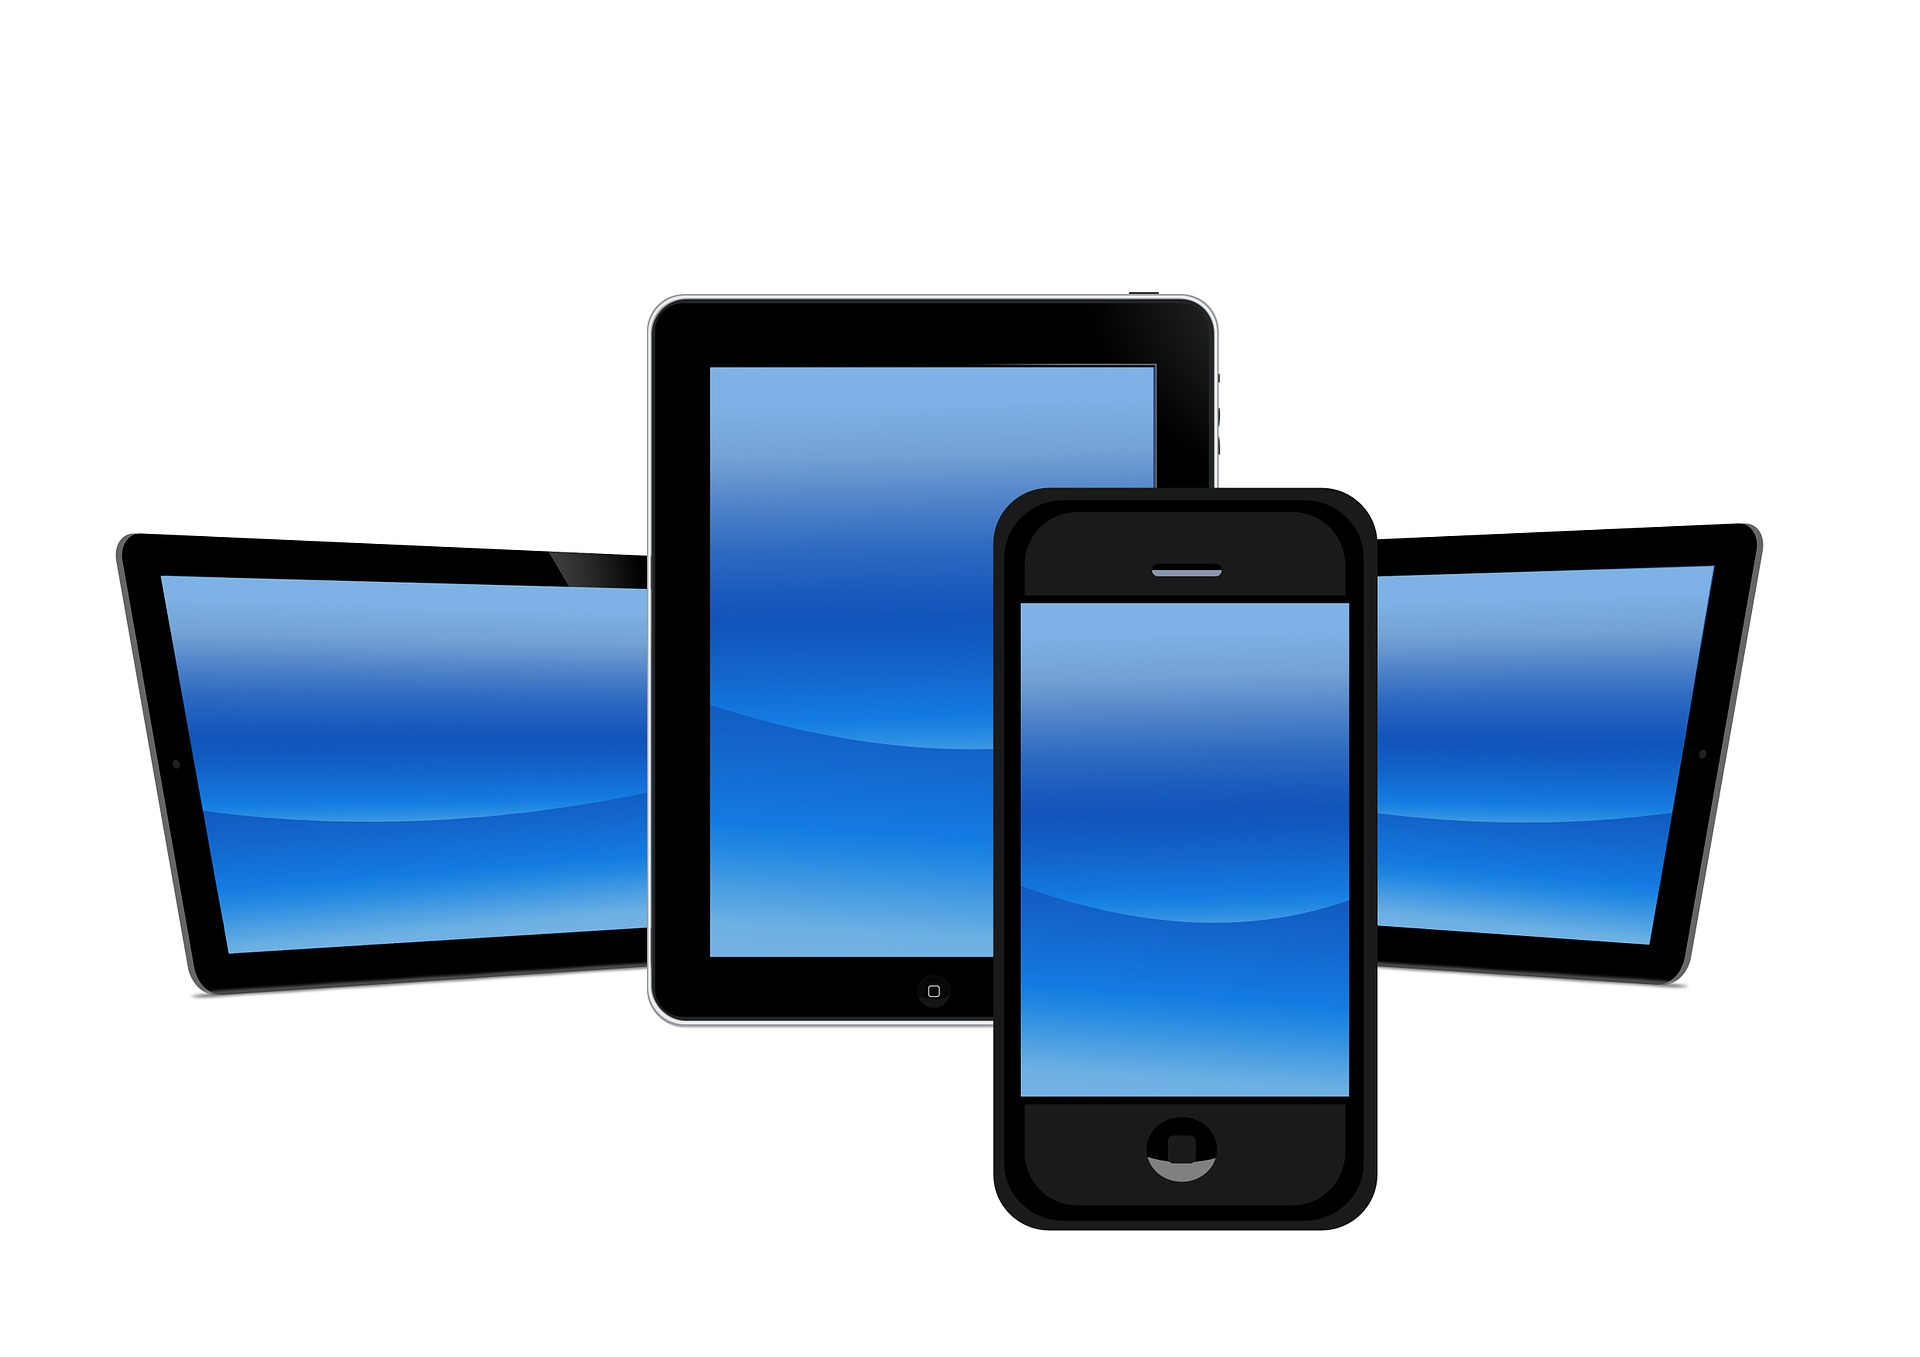
\includegraphics[scale=0.04]{images/mobile.jpg}
      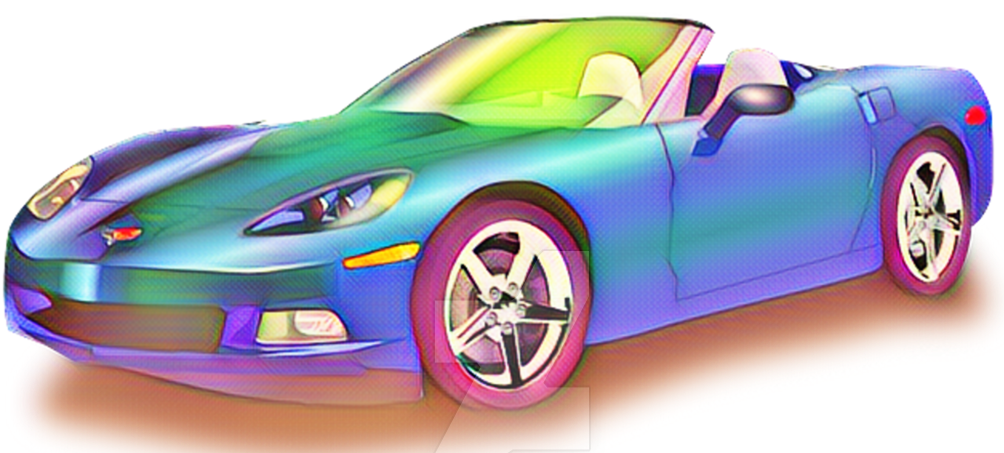
\includegraphics[scale=0.4]{images/car.png}
      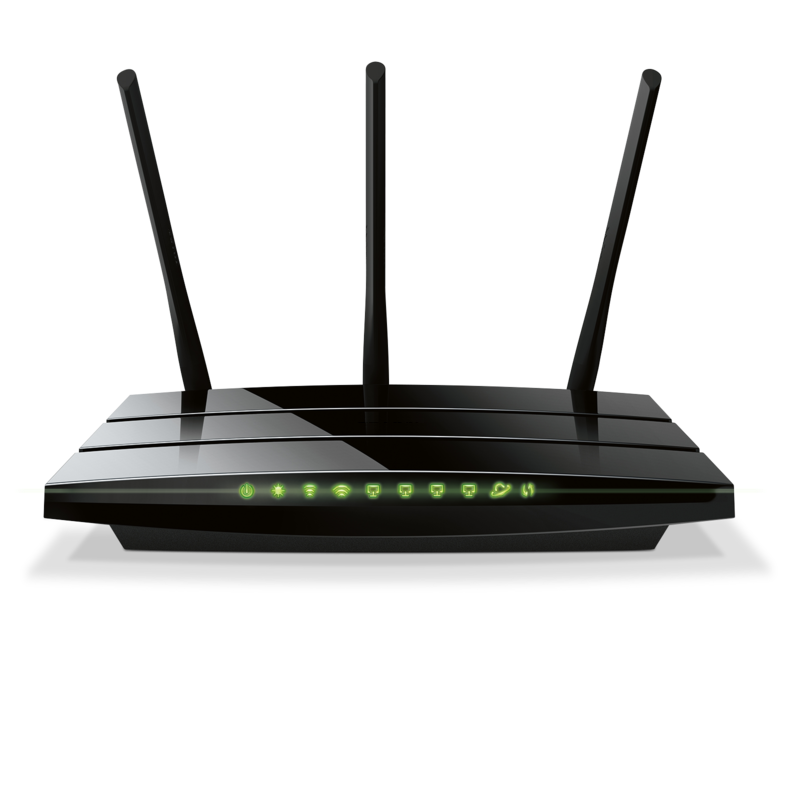
\includegraphics[scale=0.1]{images/router.png}
      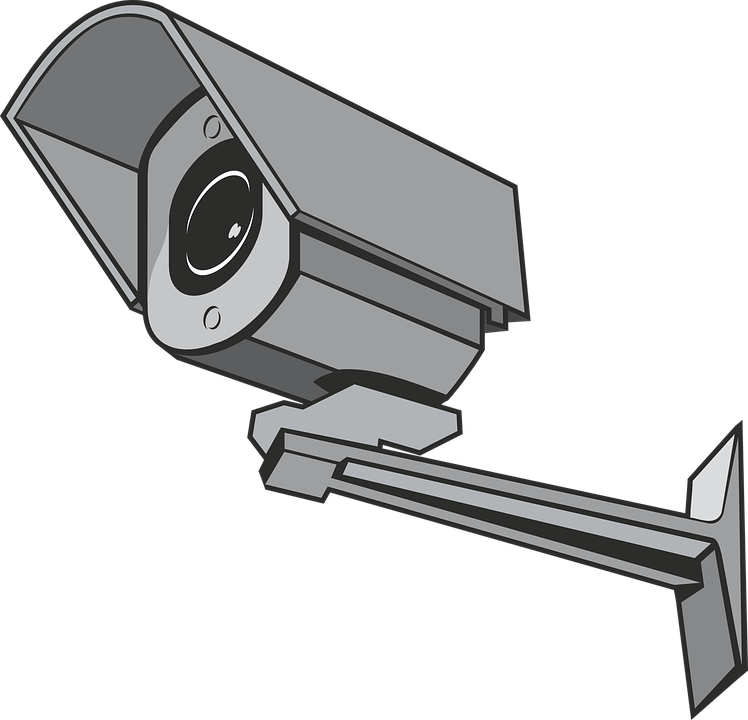
\includegraphics[scale=0.05]{images/surveillance-camera.png}
      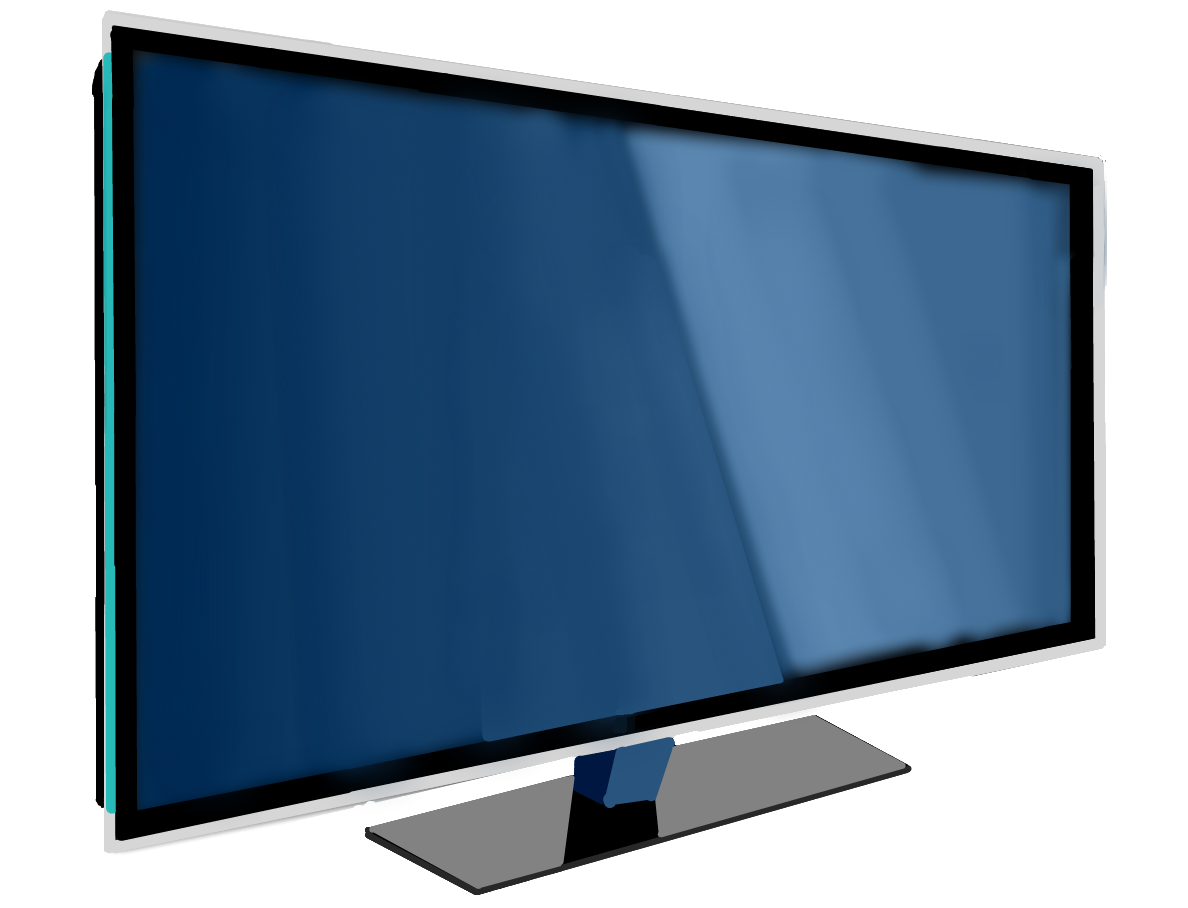
\includegraphics[scale=0.07]{images/tv.png}
      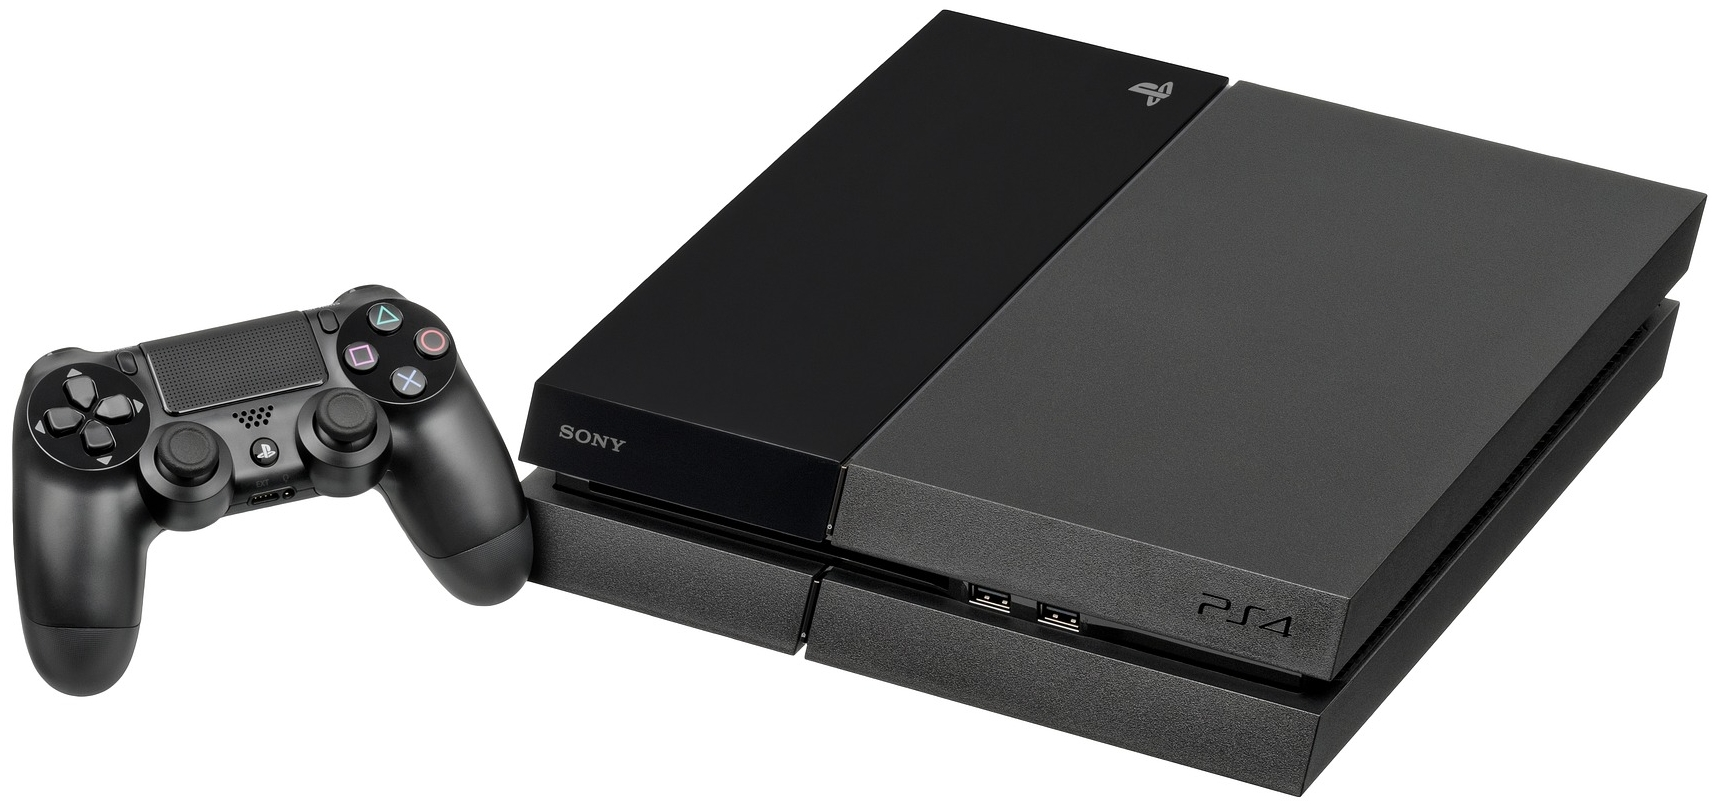
\includegraphics[scale=0.2]{images/game-console.jpg}
      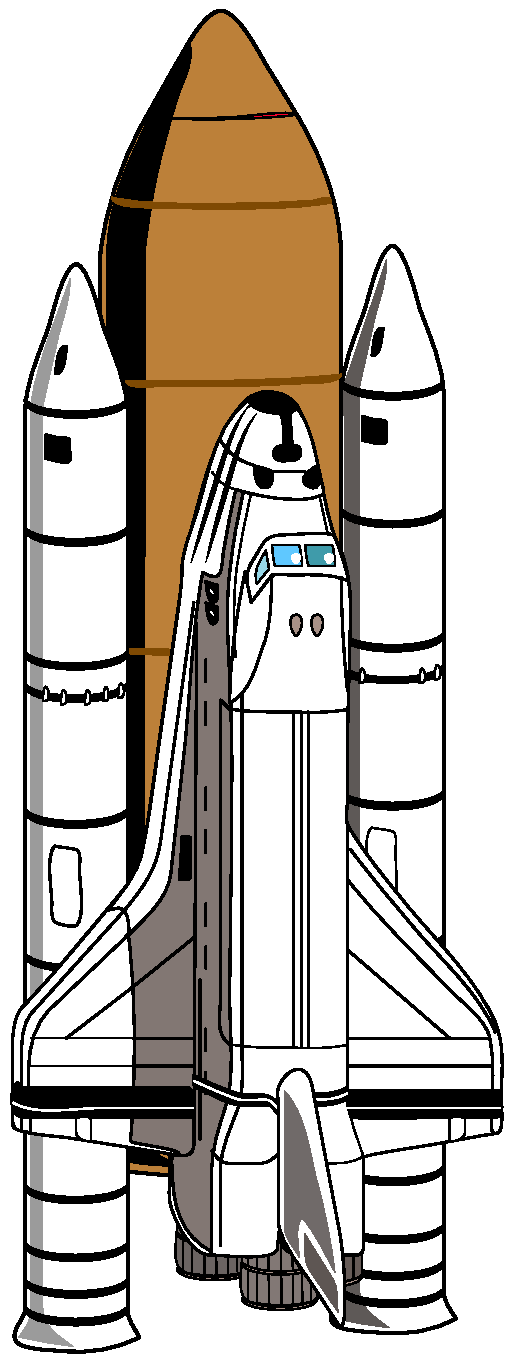
\includegraphics[scale=0.13]{images/shuttle.pdf}
      \centering
    \end{figure}
  \end{columns}
\end{frame}

\begin{frame}
  \frametitle{Embedded Programming}
  \begin{columns}
    \column{0.5\textwidth}
      Differences from regular system:
      \begin{itemize}
        \item Cross-compiling
        \item Flashing
        \item Serial console
        \item Testing concerns
        \item Working with hardware
        \item Non discoverable buses on board (device tree, platform drivers)
      \end{itemize}
    \column{0.5\textwidth}
      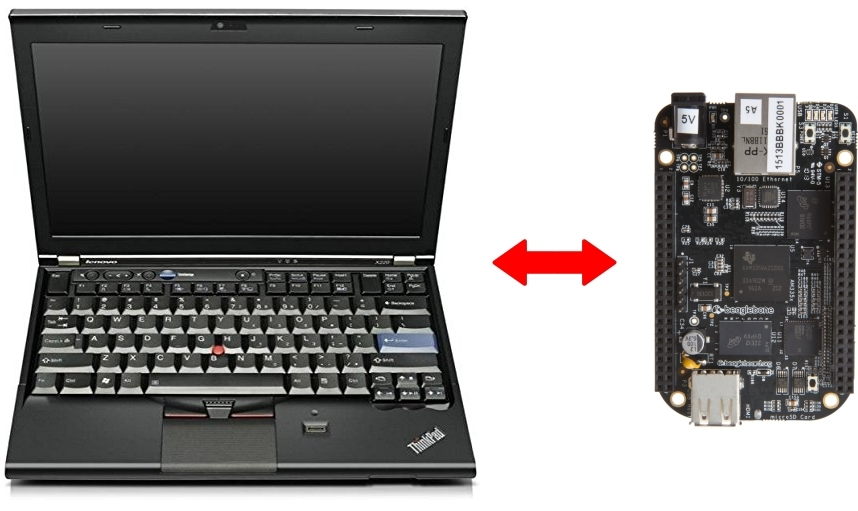
\includegraphics[scale=0.27]{images/host-target.jpg}
  \end{columns}
\end{frame}

\begin{frame}
  \frametitle{Kernel: Big Picture}
  \vspace*{-5mm} % to reduce too much whitespace after figure block
  \begin{figure}
    \centering
    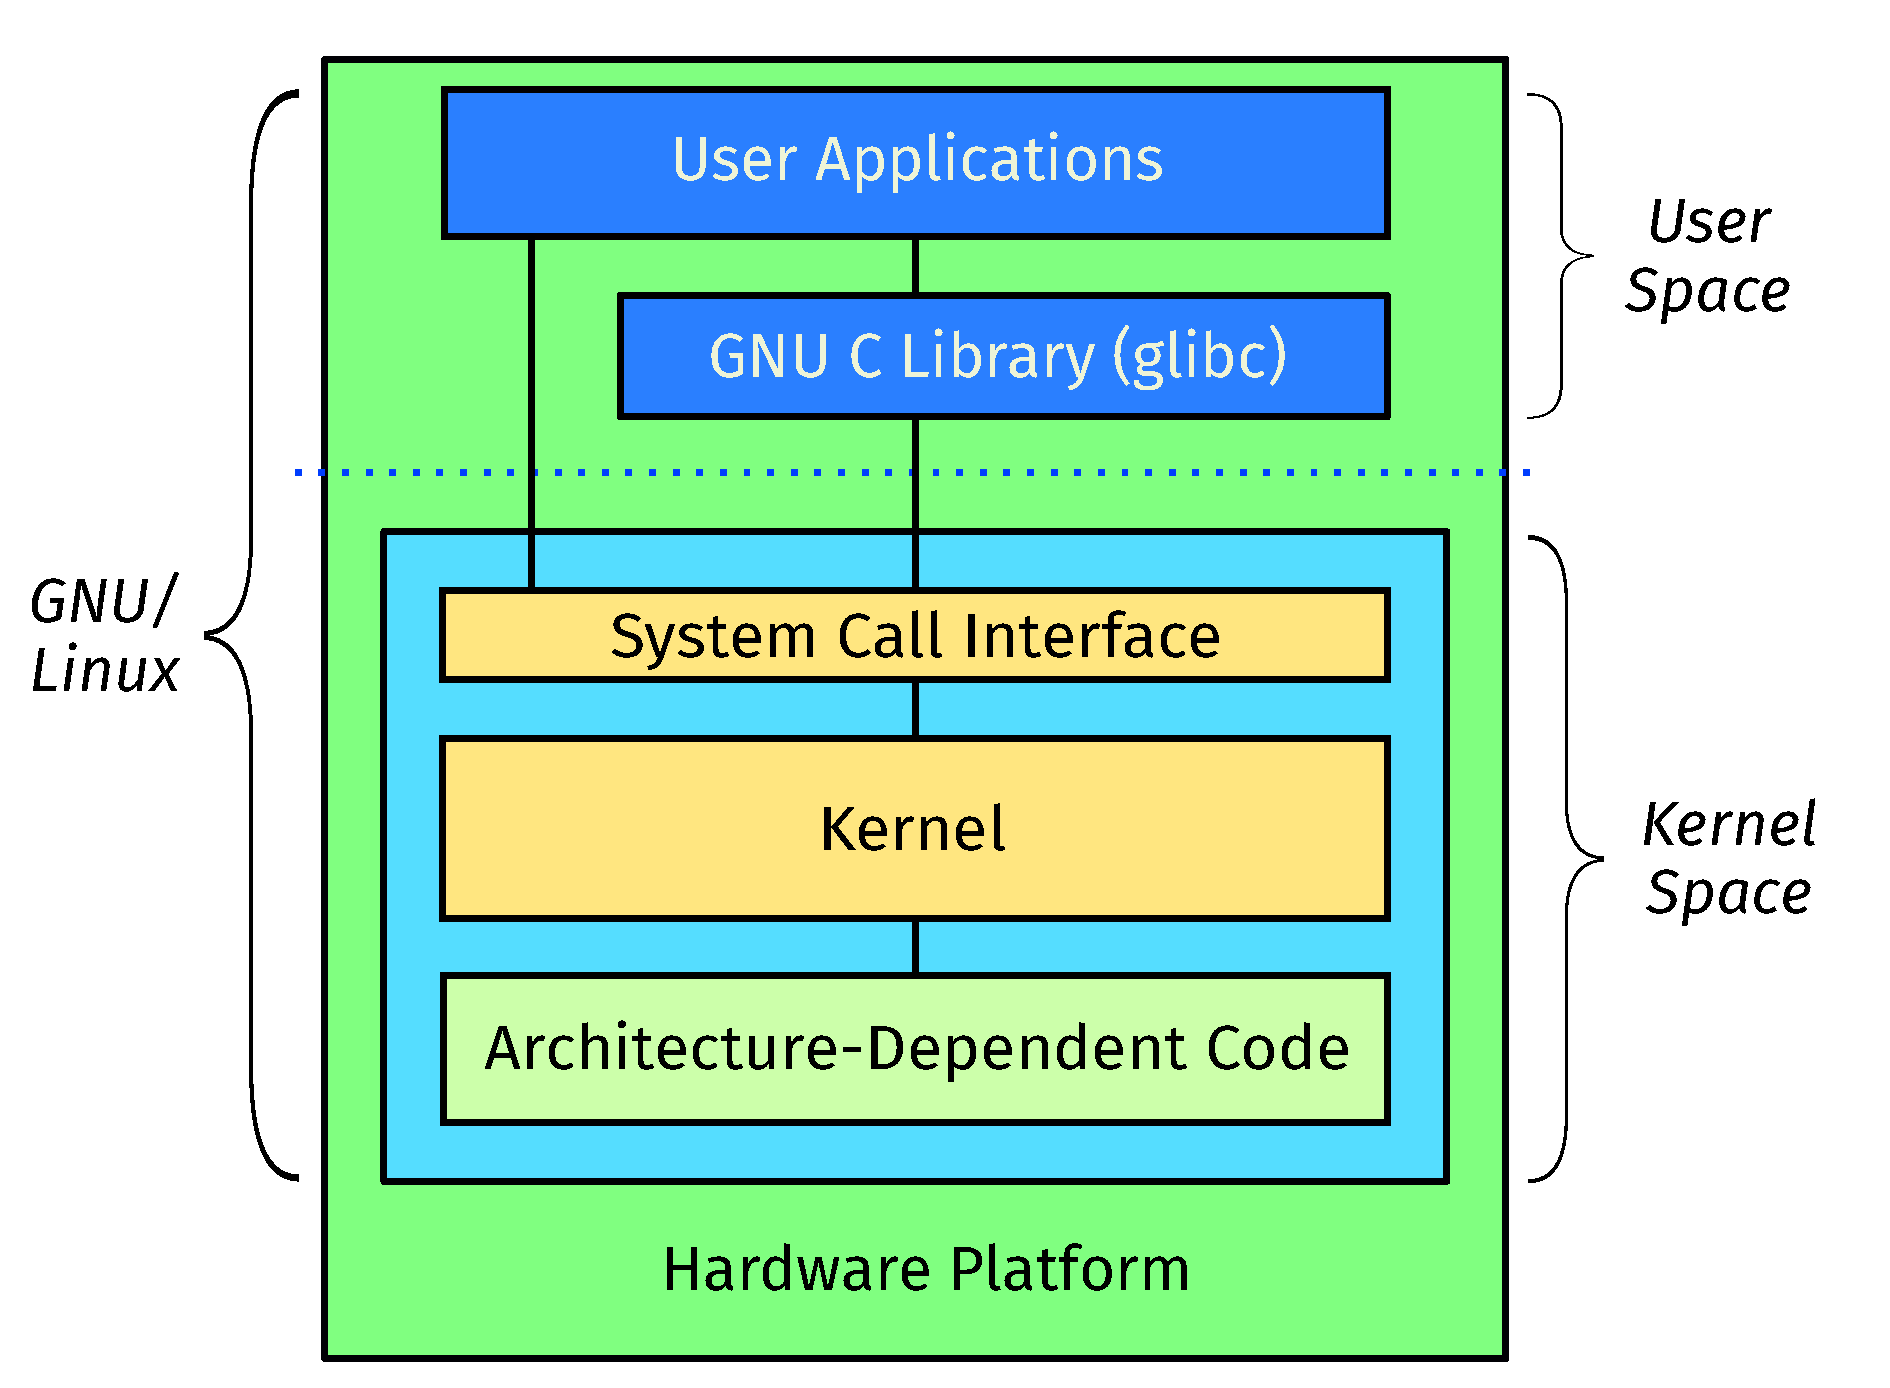
\includegraphics[scale=0.24]{images/linux-architecture.pdf}
    \caption{The fundamental architecture of the GNU/Linux operating system}
  \end{figure}
  \vspace*{-5mm} % to reduce too much whitespace after figure block
\end{frame}

\begin{frame}
  \frametitle{ARM Cortex A/R/M Families}
  \begin{figure}
    \centering
    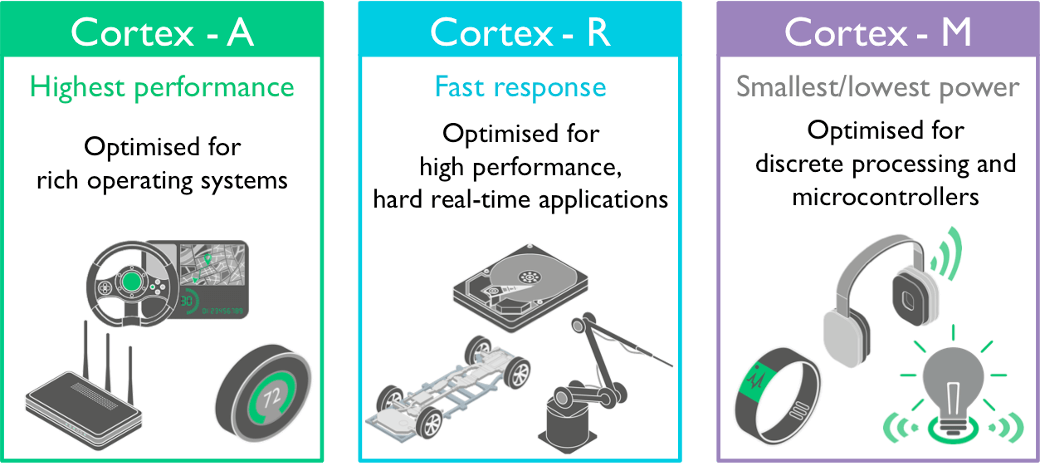
\includegraphics[scale=0.3]{images/cortex-families.png}
    \caption{ARM Cortex Processor Families}
  \end{figure}
\end{frame}

\begin{frame}
  \frametitle{AM335x SoC}
  \begin{columns}
    \column{0.5\textwidth}
      \begin{figure}
        \centering
        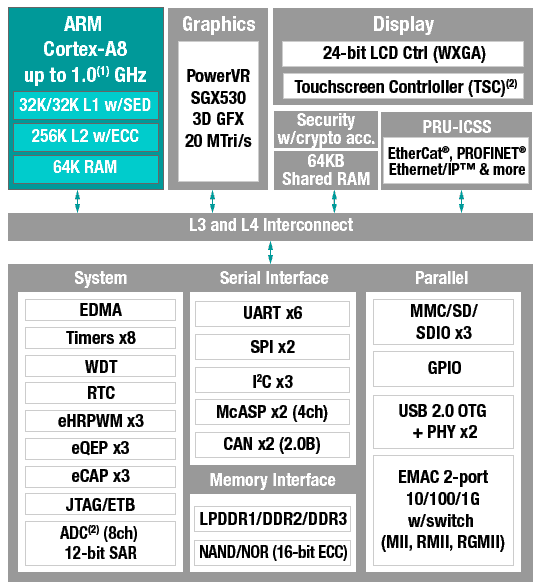
\includegraphics[scale=0.4]{images/am335x.png}
        \caption{AM335x Functional Diagram}
      \end{figure}
      \vspace*{-12mm} % to reduce too much whitespace after figure block
    \column{0.5\textwidth}
      \begin{figure}
        \centering
        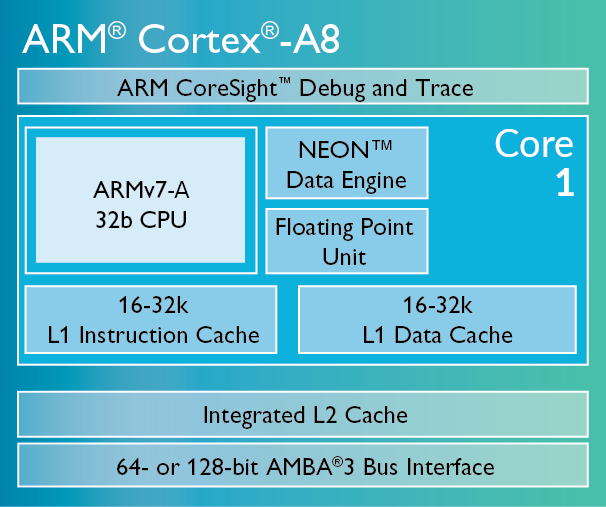
\includegraphics[scale=1]{images/cortex-a8.png}
        \caption{Cortex-A8 Processor Architecture}
      \end{figure}
  \end{columns}
\end{frame}

\begin{frame}
  \frametitle{BeagleBone Black}
  \begin{center}
    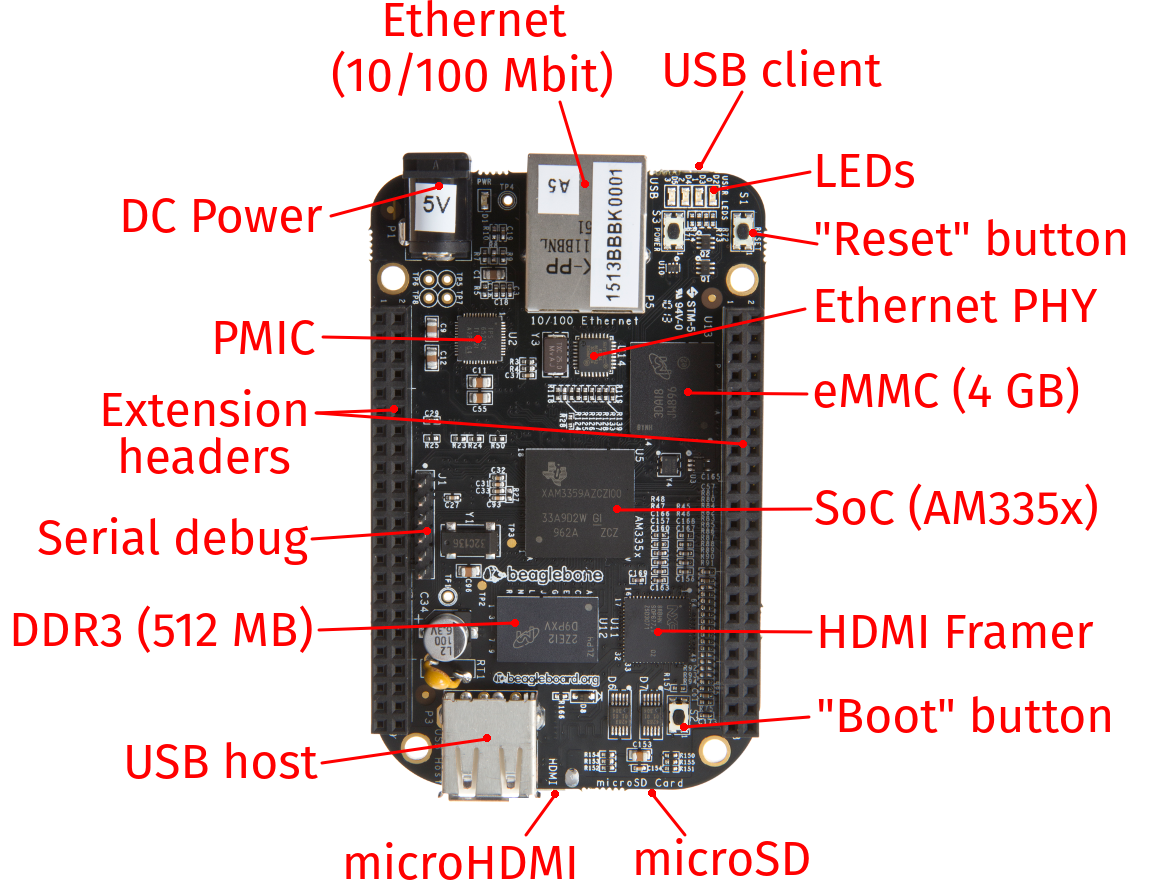
\includegraphics[scale=0.82]{images/bbb02.png}
  \end{center}
\end{frame}

\begin{frame}
  \frametitle{BeagleBone Black: Pros and Cons}
  \begin{columns}[t]
    \column{0.5\textwidth}
    Pros:
    \begin{itemize}
    \item Open Hardware
      \begin{itemize}
      \item Public TRM
      \item Schematic
      \item PCB files
      \end{itemize}
    \item Supported in upstream
      \begin{itemize}
      \item Kernel
      \item U-Boot
      \end{itemize}
    \item Conventional ARM architecture
    \item Very popular
    \item Low cost (\$55)
    \end{itemize}

    \column{0.5\textwidth}
    Cons:
    \begin{itemize}
    \item Old 32-bit architecture
    \item Single core processor
    \item Android is not supported officially
    \item No WiFi
    \end{itemize}
  \end{columns}
\end{frame}

\section{Software Overview}

\begin{frame}
  \frametitle{Software Components}
  \begin{itemize}
    \item U-Boot
    \item Linux kernel
    \item BusyBox
  \end{itemize}
  \bigskip
  \begin{overlayarea}{\textwidth}{.4\textheight}
      \only<2>{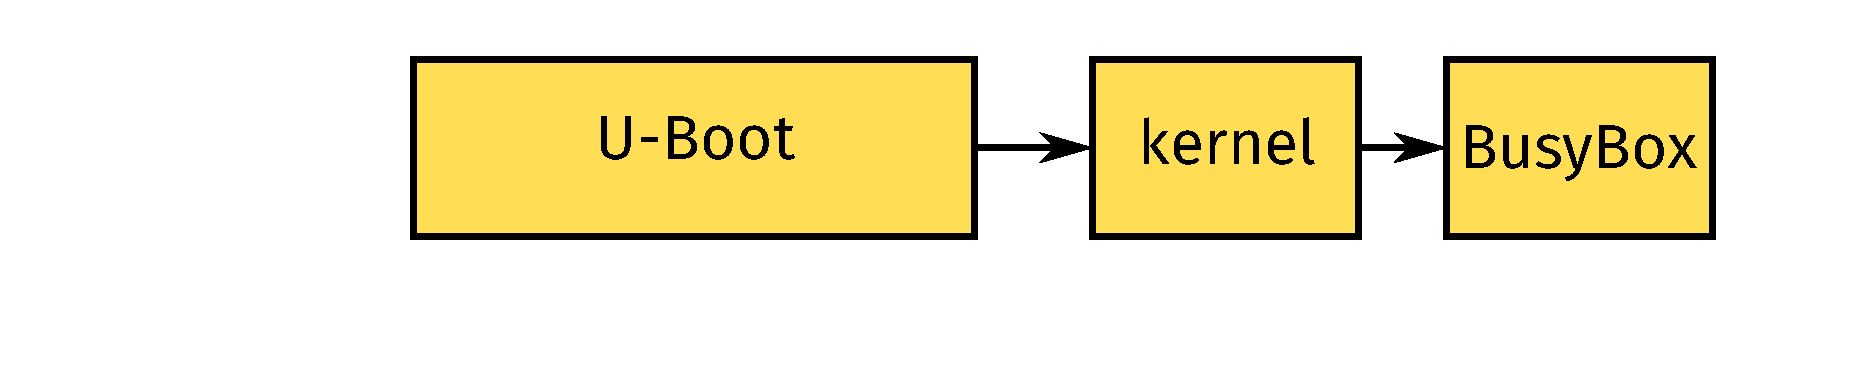
\includegraphics[scale=0.4]{images/boot1.pdf}}
      \only<3>{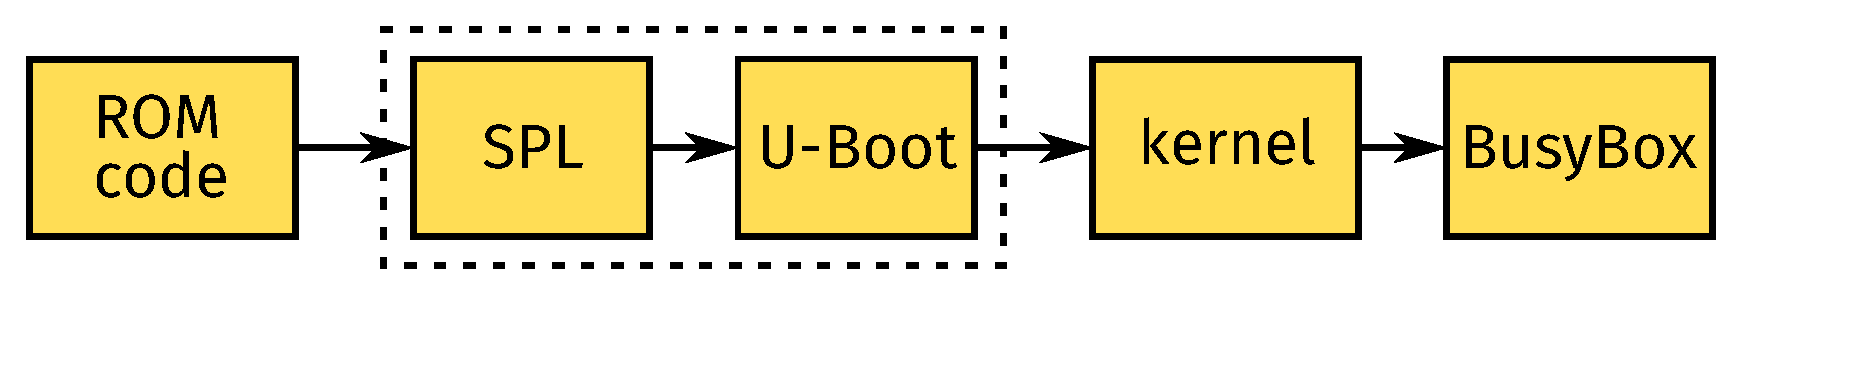
\includegraphics[scale=0.4]{images/boot2.pdf}}
      \only<4>{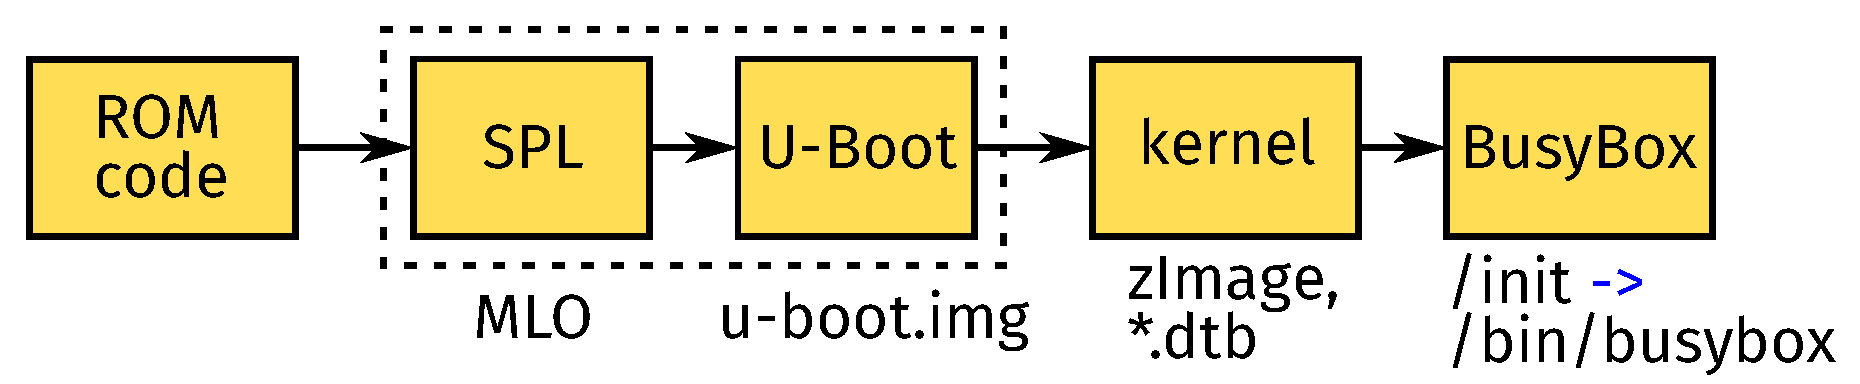
\includegraphics[scale=0.4]{images/boot3.pdf}}
  \end{overlayarea}
\end{frame}

\begin{frame}
  \frametitle{Building Steps}
  \begin{enumerate}
    \item Obtain the software
    \item Checkout to desired branch or tag
    \item Consult with \texttt{README} and \texttt{INSTALL}
    \item Install all build dependencies
    \item Configure shell environment for cross-compiling
    \item \textbf{Configure the software for build with options you desire}
    \item \textbf{Build the software}
    \item \textbf{Install/flash the built software}
  \end{enumerate}
\end{frame}

\section{Perspective on Building}

\subsection{Git Concerns}

\begin{frame}
  \frametitle{Kernel Branching Strategy}
  \begin{overlayarea}{\textwidth}{\textheight}
    \begin{figure}
      \centering
      \only<1>
      {%
      \includegraphics[scale=0.5]{images/branching-strategy1.pdf}%
      }%
      \only<2>
      {%
      \includegraphics[scale=0.5]{images/branching-strategy2.pdf}%
      }%
    \end{figure}
  \end{overlayarea}
  \vspace*{-10mm}
\end{frame}

\begin{frame}
  \frametitle{Stable Trees}
  \begin{itemize}
    \item Git tags: for releases (e.g. \texttt{v4.19})
    \item Git branches: for stable releases (e.g. \texttt{linux-4.19.y})
    \item Some stable branches are LTS (Long Term Support)
    \item When possible, let's use stable branches (for reliability)
    \item When stable branches are not available, let's use release tags
  \end{itemize}
\end{frame}

\subsection{Toolchain}

\begin{frame}
  \frametitle{Toolchain (page 1)}
  \begin{center}
    \includegraphics[width=0.8\textwidth]{images/cross-toolchain.pdf}
  \end{center}
\end{frame}

\begin{frame}
  \frametitle{Toolchain (page 2)}
  \begin{itemize}
    \item Set of tools for cross-compiling:
    \begin{enumerate}
      \item \texttt{gcc}
      \item binutils: \texttt{ld}, \texttt{as}, \texttt{objdump},
            \texttt{objcopy}, \texttt{readelf}, etc.
      \item \texttt{glibc} and other system libraries (\alert{optional})
      \item Linux kernel headers (\alert{optional})
      \item \texttt{gdb} (\alert{optional})
    \end{enumerate}
    \pause
    \item Toolchain types:
    \begin{itemize}
      \item Bare-metal targeted (\texttt{arm-eabi}): for U-Boot and kernel
      \item Linux targeted (\texttt{arm-linux-gnueabihf}): for BusyBox
    \end{itemize}
    \item In our case: host = x86\_64, target = ARMv7-A
    \item We use only GNU (GCC-based) toolchains
  \end{itemize}
\end{frame}

\begin{frame}
  \frametitle{Toolchain (page 3)}
  Toolchain tuple examples:
  \begin{itemize}
  \item \textbf{arm-foo-none-eabi}, bare-metal toolchain targeting the ARM
        architecture, from vendor \textit{foo}
  \item \textbf{arm-unknown-linux-gnueabihf}, Linux toolchain targeting the ARM
        architecture, using the EABIhf ABI and the glibc C library, from an
        \textit{unknown} vendor
  \item \textbf{armeb-linux-uclibcgnueabi}, Linux toolchain targeting the ARM
        big-endian architecture, using the EABI ABI and the uClibc C library
  \item \textbf{mips-img-linux-gnu}, Linux toolchain targeting the MIPS
        architecture, using the glibc C library, provided by Imagination
        Technologies
  \end{itemize}
\end{frame}

\begin{frame}[fragile]
  \frametitle{Toolchain (page 4)}
  \begin{itemize}
  \item Regular compilation on host system (using \textit{native toolchain}):
  \begin{Verbatim}
$ gcc main.c
  \end{Verbatim}
  \pause
  \vspace*{5mm}
  \item Cross-compilation for ARM target (part before \texttt{gcc} is called
        \textit{prefix}):
  \begin{Verbatim}[commandchars=\\\{\}]
$ \textcolor{green}{/toolchain/path/bin/}\textcolor{red}{arm-eabi-}gcc main.c
  \end{Verbatim}
  \pause
  \vspace*{5mm}
  \item More universal way:
  \begin{Verbatim}[commandchars=\\\{\}]
$ PATH=\textcolor{green}{/toolchain/path/bin}:$PATH
$ CROSS_COMPILE=\textcolor{red}{arm-eabi-}
$ $\{CROSS_COMPILE\}gcc main.c
  \end{Verbatim}
  \end{itemize}
\end{frame}

\begin{frame}[fragile]
  \frametitle{Specifying Architecture}
  \begin{itemize}
    \item Kernel supports many CPU architectures:
    \begin{Verbatim}[commandchars=\\\{\}]
linux/
├── \colorbox{pink}{arch/}               -- \colorbox{pink}{platform-dependent code}
│   ├── arm/
│   ├── arm64/
│   ├── x86/
│   └── ...
└── \colorbox{green}{drivers/}            -- \colorbox{green}{platform-independent code}
    \end{Verbatim}
    \bigskip
    \item We need to choose which architecture to build for:
    \begin{verbatim}
$ export ARCH=arm
    \end{verbatim}
  \end{itemize}
\end{frame}

\begin{frame}[fragile]
  \frametitle{Shell Environment}
  \begin{itemize}
  \item Shell environment configuration for building U-Boot/kernel/BusyBox:
  \begin{verbatim}
$ export ARCH=arm
$ export PATH=/toolchain/path/bin:$PATH
$ export CROSS_COMPILE=arm-eabi-
  \end{verbatim}
  \item Makefile utilizes those env vars
  \end{itemize}
\end{frame}

\begin{frame}[standout]
  Take Five
\end{frame}

\subsection{Kbuild: User's Perspective}

\begin{frame}[standout]
  Kbuild: User's Perspective
\end{frame}

\begin{frame}[fragile]
  \frametitle{Building: General Steps}
  \begin{itemize}
    \item All projects (U-Boot, Linux kernel and BusyBox) use Kbuild
    \item Build steps: configuration, build, installation
    \item \alert{Configuration} (generate \texttt{.config} file):
    \begin{verbatim}
$ make defconfig
    \end{verbatim}
    \item \alert{Build}:
    \begin{verbatim}
$ make
    \end{verbatim}
    \item \alert{Installation}:
    \begin{verbatim}
$ make install
    \end{verbatim}
    \vspace*{-2mm} % to reduce too much whitespace after verbatim block
  \end{itemize}
\end{frame}

\begin{frame}[fragile]
  \frametitle{Building: Custom Configuration}
  \begin{itemize}
  \item Sometimes existing \texttt{defconfig} is not enough
  \item How can we customize our configuration?
    \begin{itemize}
      \item Using \texttt{make menuconfig}
      \item Using \texttt{merge\_config.sh} script
      \item Using old \texttt{.config} file
    \end{itemize}
  \pause
  \bigskip
  \item Example: kernel configuration using \texttt{merge\_config.sh}:
  \begin{verbatim}
$ ./scripts/kconfig/merge_config.sh   \
  arch/arm/configs/multi_v7_defconfig \
  fragments/bbb.cfg
  \end{verbatim}
  \vspace*{-2mm} % to reduce too much whitespace after verbatim block
  \end{itemize}
\end{frame}

\begin{frame}[fragile]
  \frametitle{Building: .config Example}
  Excerpt from \texttt{.config} file:
  \begin{Verbatim}[commandchars=\\\{\}]
CONFIG_USE_OF=\textcolor{red}{y}
CONFIG_DEFAULT_HOSTNAME=\textcolor{green}{"(none)"}
CONFIG_CMDLINE=\textcolor{green}{""}
\textcolor{gray}{# CONFIG_PREEMPT is not set}
CONFIG_I2C_GPIO=\textcolor{red}{m}
CONFIG_LOG_BUF_SHIFT=\textcolor{blue}{17}
\textcolor{gray}{# CONFIG_SLAB is not set}
CONFIG_USB=\textcolor{red}{y}
CONFIG_SND_USB_AUDIO=\textcolor{red}{m}
  \end{Verbatim}
\end{frame}

\begin{frame}
  \frametitle{Kernel Modules}
  \begin{itemize}
    \item Every driver is a module
    \item Kernel modules can be:
    \begin{itemize}
      \item Loadable: ``\texttt{=m}''
      \item Built-in: ``\texttt{=y}''
    \end{itemize}
    \item Kernel loadabe module (\texttt{.ko} file) is some code that can be
          loaded into kernel space (i.e. added to running kernel as a plugin)
    \pause
    \item How it works:
    \begin{itemize}
      \item \texttt{multi\_v7\_defconfig} is common for all ARMv7 systems (so
            the single \texttt{zImage} can be used)
      \item Device Tree file covers SoC and board differences
      \item Needed modules (for particular board) can be loaded in run-time
    \end{itemize}
    \item It's not always convenient to load a lot of modules
  \end{itemize}
\end{frame}

\begin{frame}
  \frametitle{How to Speed-Up the Build? (page 1)}
  \begin{center}
    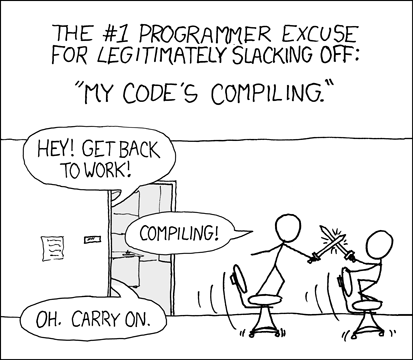
\includegraphics[scale=0.45]{images/compiling.png}
  \end{center}
\end{frame}

\begin{frame}[fragile]
  \frametitle{How to Speed-Up the Build? (page 2)}
  \begin{itemize}
    \item \alert{\textbf{Kbuild tracks all dependencies very well!}}
    \item \textit{Clean build} (try to avoid it):
    \begin{verbatim}
$ make
// Do some changes to source code
$ make distclean
$ make
    \end{verbatim}
    \item Use \textit{incremental build} instead:
    \begin{verbatim}
$ make
// Do some changes to source code
$ make
    \end{verbatim}
  \end{itemize}
  \vspace*{-3mm}
\end{frame}

\begin{frame}[fragile]
  \frametitle{How to Speed-Up the Build? (page 3)}
  \begin{itemize}
    \item Distribute the compilation between CPU cores using multi-threading build:
    \begin{verbatim}
$ make -j4
    \end{verbatim}
    \item Use \texttt{ccache} tool:
    \begin{itemize}
      \item Caches \texttt{.o} files on the first build
      \item On next build, if some \texttt{.o} files are unchanged, cached
            versions will be used
      \item \texttt{ccache} creates a hash by \texttt{.c} file content and by
            build command
      \item ...So if you change the toolchain, cache won't be used
      \item Speed up for clean build is usually ~5 times
      \item Can be used as a wrapper:
      \begin{verbatim}
$ ccache gcc main.c
      \end{verbatim}
    \end{itemize}
  \end{itemize}
\end{frame}

\begin{frame}
  \frametitle{How to Speed-Up the Build? (page 4)}
  \begin{center}
    \includegraphics[scale=0.45]{images/ccache.png}
  \end{center}
  \vspace*{-10mm}
\end{frame}

\begin{frame}
  \frametitle{How to Speed-Up the Build? (page 5)}
  \begin{center}
    
\includegraphics[scale=0.55]{images/nickel.png}
  \end{center}
\end{frame}

\subsection{RootFS}

\begin{frame}[standout]
  RootFS
\end{frame}

\begin{frame}
  \frametitle{RootFS}
  What is RootFS?
  \begin{itemize}
  \item Filesystem that is needed to make userspace work
  \item Mounted to ``/''
  \item Crucial component is \texttt{init} tool
  \item Besides of that: libc, kernel modules, tools, config files...
  \end{itemize}
  \pause
  Known rootfs's for BBB:
  \begin{itemize}
  \item Debian
  \item Yocto/OpenEmbedded
  \item BuildRoot
  \item BusyBox
  \end{itemize}
\end{frame}

\begin{frame}
  \frametitle{BusyBox Linking: Static}
  \begin{overlayarea}{\textwidth}{\textheight}
    \begin{figure}
      \centering
      \includegraphics[scale=0.5]{images/busybox-static.pdf}
    \end{figure}
  \end{overlayarea}
  \vspace*{-10mm}
\end{frame}

\begin{frame}
  \frametitle{BusyBox Linking: Dynamic}
  \begin{overlayarea}{\textwidth}{\textheight}
    \begin{figure}
      \centering
      \includegraphics[scale=0.5]{images/busybox-dynamic.pdf}
    \end{figure}
  \end{overlayarea}
  \vspace*{-10mm}
\end{frame}

\begin{frame}
  \frametitle{BusyBox Linking: Static vs Dynamic}
  \begin{itemize}
    \item \alert{Static linking}: libc (.a) is compiled in your binary
      \begin{itemize}
        \item Only ``\texttt{busybox}'' binary is needed in rootfs
        \item Easier to build and minimal
        \item Some networking functions won’t work (like \texttt{nslookup},
              see libnss)
      \end{itemize}
    \bigskip
    \item \alert{Dynamic linking}: libc used as a shared library (.so)
      \begin{itemize}
        \item Only one copy of libc is used (for all possible apps)
        \item Dynamic libraries must be copied in rootfs \texttt{/lib}
              (libc and its dependencies)
      \end{itemize}
  \end{itemize}
\end{frame}

\begin{frame}[fragile]
  \frametitle{BusyBox Applets}
  \begin{itemize}
  \item BusyBox is a multi-call binary
  \item Apps in BusyBox rootfs are just symbolic links:
    \begin{Verbatim}[commandchars=\\\{\}]
\textcolor{blue}{/bin}
├── \textcolor{green}{busybox}
├── \textcolor{cyan}{grep} -> \textcolor{green}{busybox}
└── \textcolor{cyan}{ls}   -> \textcolor{green}{busybox}
    \end{Verbatim}
  \item So you can call \textbf{ls} tool like this:
    \begin{Verbatim}
# busybox ls -l
    \end{Verbatim}
  \item ...which is identical to this form:
    \begin{Verbatim}
# ls -l
    \end{Verbatim}
  \end{itemize}
\end{frame}

\begin{frame}
  \frametitle{Init process}
  \begin{itemize}
  \item First process started during boot (kernel starts it)
  \item PID = 1, uid = 0 (root)
  \item It never exits (daemon)
  \item Init is a parent for all processes
  \item Automatically adopts all orphaned processes
  \item Init is started by the kernel using a hard-coded filename (e.g. \texttt{/init})
  \item A kernel panic will occur if the kernel is unable to start it
  \item Most popular init implementations:
    \begin{itemize}
    \item sysvinit
    \item openrc
    \item upstart
    \item systemd
    \end{itemize}
  \end{itemize}
  \vspace*{-5mm}
\end{frame}

\begin{frame}
  \frametitle{BusyBox init}
  \begin{itemize}
  \item \texttt{busybox} tool implements init as an applet
  \item BusyBox's init implementation resembles SysVinit, but more simple
  \item Doesn't support runlevels (as opposed to SysVinit)
  \item Starts \texttt{/etc/init.d/rcS} script
  \item (Re)spawns children according to \texttt{/etc/inittab} (e.g. \textbf{getty})
  \item Handles signals (e.g. \textbf{reboot} and \textbf{poweroff})
  \end{itemize}
\end{frame}

\begin{frame}
  \frametitle{BusyBox init (cont'd)}
  \vspace*{-3mm}
  \begin{center}
    \includegraphics[scale=0.37]{images/busybox-init.pdf}
  \end{center}
  \vspace*{-10mm}
\end{frame}

\begin{frame}
  \frametitle{BusyBox Device Manager}
  \begin{itemize}
    \item No \texttt{udev} in BusyBox
    \item \textit{`mdev is a mini-udev implementation for dynamically creating
                  device nodes in the /dev directory'}
    \item Requires SysFS support in kernel; it must be mounted to \texttt{/sys}
    \item Can be also used for hot-plugging (e.g. load needed kernel module when
          some USB device was inserted)
    \item \texttt{mdev -s}: scan \texttt{/sys} and populate \texttt{/dev}
    \item \texttt{mdev} without params: kernel hotplug helper
    \item For more details see: \texttt{doc/mdev.txt}
  \end{itemize}
\end{frame}

\begin{frame}[fragile]
  \frametitle{BusyBox init: Script Example}
  \begin{itemize}
    \item \texttt{rc} = ``run commands'', \texttt{S} = single-user runlevel
    \item Example of \texttt{/etc/init.d/rcS} file:
    \vspace{3mm}
    \hrule
    \vspace{3mm}
    \begin{verbatim}
#!/bin/sh

mount -t sysfs none /sys
mount -t proc none /proc
mount -t debugfs none /sys/kernel/debug

echo /sbin/mdev > /proc/sys/kernel/hotplug
mdev -s
    \end{verbatim}
  \end{itemize}
\end{frame}

\begin{frame}[fragile]
  \frametitle{BusyBox rootfs (static, minimal)}
  \begin{columns}
    \column{0.5\textwidth}
      \begin{Verbatim}[commandchars=\\\{\}]
\textcolor{blue}{/}
├── \textcolor{blue}{bin}
│   └── \textcolor{green}{busybox}
├── \textcolor{blue}{boot}
│   ├── am335x-boneblack.dtb
│   └── \textcolor{green}{zImage}
├── \textcolor{blue}{dev}
├── \textcolor{blue}{etc}
│   └── \textcolor{blue}{init.d}
│       └── \textcolor{green}{rcS}
      \end{Verbatim}
    \column{0.5\textwidth}
      \begin{Verbatim}[commandchars=\\\{\}]
├── \textcolor{cyan}{init} -> \textcolor{green}{bin/busybox}
├── \textcolor{cyan}{linuxrc} -> \textcolor{green}{bin/busybox}
├── \textcolor{blue}{proc}
├── \textcolor{blue}{root}
├── \textcolor{blue}{sbin}
├── \textcolor{blue}{sys}
├── \textcolor{blue}{tmp}
└── \textcolor{blue}{usr}
    ├── \textcolor{blue}{bin}
    └── \textcolor{blue}{sbin}
      \end{Verbatim}
  \end{columns}
\end{frame}


\begin{frame}[standout]
  Demo: menuconfig
\end{frame}

\section*{Assignments}

\begin{frame}
  \frametitle{Assignment}
  \begin{itemize}
    \item Using BBB instructions guide (will be sent out):
      \begin{itemize}
        \item Go through 1st chapter (``Preparing the Tools'')
        \item Go through 2nd chapter (``Obtaining and Building the Software'')
        \item Run built software on QEMU, using section 3.1 ``QEMU Boot''
      \end{itemize}
    \item Download TRM and datasheet for AM335x
    \item Download schematic for BBB
    \item Proof: send me screenshot of \texttt{uname -a} output in your QEMU
  \end{itemize}
\end{frame}

\begin{frame}
  \frametitle{Advanced assignment (optional)}
  \begin{itemize}
    \item Using TRM, figure out:
      \begin{itemize}
        \item Which module (TRM section?) is used for setting clocks (gating, DPLL)
        \item Which module (TRM section?) is used for pin multiplexing
        \item Where GPIO output registers are documented
        \item Where UART RX/TX registers are documented
      \end{itemize}
    \item Using schematic, figure out:
      \begin{itemize}
        \item Which pins (pads) the user LEDs are connected to
        \item How to mux those pins for GPIO (use datasheet and TRM)?
        \item Which registers to use for pin muxing and then blinking some LED?
      \end{itemize}
  \end{itemize}
\end{frame}

\section*{References}

\begin{frame}
  \frametitle{Recommended Reading}
  \begin{thebibliography}{}
  \setbeamertemplate{bibliography item}[book]
    \bibitem{Embedded2008}
      Karim Yaghmour, Jon Masters and others.
      \newblock \emph{Building Embedded Linux Systems}.
    \bibitem{Linux2014}
      Brian Ward.
      \newblock \emph{How Linux Works}, 2nd Edition.
    \bibitem{ARM}
      Andrew N. Sloss and others.
      \newblock \emph{ARM System Developer's Guide}.
    \bibitem{LKD3}
      Robert Love.
     \newblock \emph{Linux Kernel Development}, 3rd Edition.
  \end{thebibliography}
\end{frame}

\begin{frame}[standout]
  Thank you!
\end{frame}

\end{document}
